% Experiment

\chapter{Experimental Setup}
\label{ch:experimental-setup}

For the experimentation phase we have used a Intel Core i7-6700HQ CPU
@ 2.60GHz, with 16GB of RAM, and a Cuda enabled Nvidia GeForce GTX
960M graphic card.

The data-set previously described in \autoref{part:variables} has been
pre-processed. This process consisted in narrowing down the data to
the same date range. Later the missing values where filled with
interpolated values. Finally the data-set has been normalized using a
standard score described in \autoref{eq:standard-score}.

\begin{equation}
  \begin{aligned}
    \label{eq:standard-score} X_{norm} & = \frac{X-\mu}{\sigma} \\
X_{norm} & \leftarrow \text{Normalized instance} \\ X & \leftarrow
\text{Original instance} \\ \mu & \leftarrow \text{Feature mean} \\
\sigma & \leftarrow \text{Feature standard deviation} \\
  \end{aligned}
\end{equation}

After predicting the values of the BTC price, the values are still
normalized. In order to correctly interpret them and compute the error
measures, this prediction has been de-normalized using the inverse
function of \autoref{eq:standard-score}, which is represented in
\autoref{eq:inverse-standard-score}.

\begin{equation}
  \begin{aligned}
    \label{eq:inverse-standard-score} \hat{X} & = \hat{X}_{norm}
\times \sigma + \mu \\ \hat{X}_{norm} & \leftarrow \text{Normalized
prediction} \\ \hat{X} & \leftarrow \text{De-normalized prediction} \\
\mu & \leftarrow \text{Feature mean} \\ \sigma & \leftarrow
\text{Feature standard deviation} \\
  \end{aligned}
\end{equation}

After the pre-processing, and to avoid over-fitting we have used
\textit{time series cross-validation} proposed by
\cite{robjhyndman2010}. The particular implementation of this
technique used uses a test partition of size 1, which we call $x_{t +
1}$ and a train partition composed of all the elements from the
$1095$-th to the $t$-th. The details about why we used $1095$-th as
the first element and the overall technique can be found in
\autoref{part:implementation}.

The layout of the network is the \textit{fully connected recurrent
neural network} which is shown in \autoref{fig:rnn-topology}.

\begin{figure}[bth] \myfloatalign
{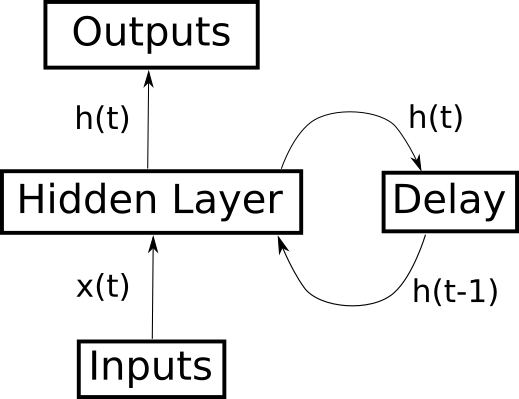
\includegraphics[width=.5\linewidth] {gfx/rnn-topology}}
  \caption{\textit{RNN} topology.}
  \label{fig:rnn-topology}
\end{figure}

The first layer is composed of 1 neuron per instance, the hidden layer
is composed of another neuron per instances, and the output is
composed of only one neuron. More details related to \textit{RNNs} can
be found in \autoref{part:method-technique}.

\chapter{Experimental Results}
\label{ch:experimental-results}

In this section we present the results of the experiments performed.
We decided that we would compare the performance of \textit{RNN} with
a traditional method such as \textit{VAR}.

Both \autoref{fig:predictions-subplots} and \autoref{fig:predictions}
represent a day ahead prediction of the Bitcoin price, compared to the
actual Bitcoin price, shown in the variable \textit{MarketPrice}. Is
the same information presented in two different ways to allow the
viewer to see the particular values of each one in
\autoref{fig:predictions-subplots}, and, on the other side, to be able
to compare closely the values of the two models and
\textit{MarketPrice} the viewer can use \autoref{fig:predictions}.

\begin{figure}[bth] \myfloatalign {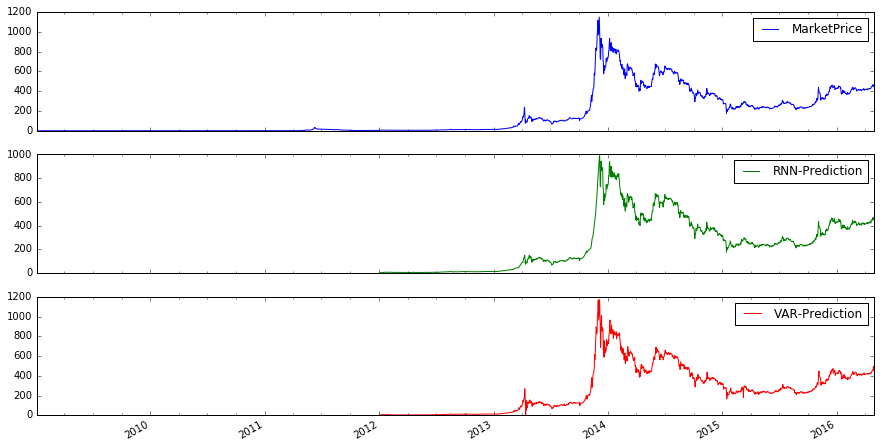
\includegraphics[width=1\linewidth]
{gfx/predictions-subplots}}
  \caption{Predictions models and \textit{MarketPrice} true values in
separate charts.}
  \label{fig:predictions-subplots}
\end{figure}

Although the shapes of the charts are similar, it can be noticed how
\textit{RNN} takes more instances to learn certain patterns, like the
one present in the first quarter of 2013, where \textit{RNN} doesn't
have the spike that \textit{VAR} and \textit{MarketPrice} do have.

It can also be noticed in \autoref{fig:predictions} that \textit{RNN}
has a delay compared to \textit{VAR} and \textit{MarketPrice}. This
can give as the intuition that \textit{RNN} learning rate is lower
than \textit{VAR}. But all this observation are mere thoughts but are
not a measure the correct measure to quantify the goodness of
prediction models and neither is a suitable technique to compare
prediction models.

\begin{figure}[bth]
  \myfloatalign {
    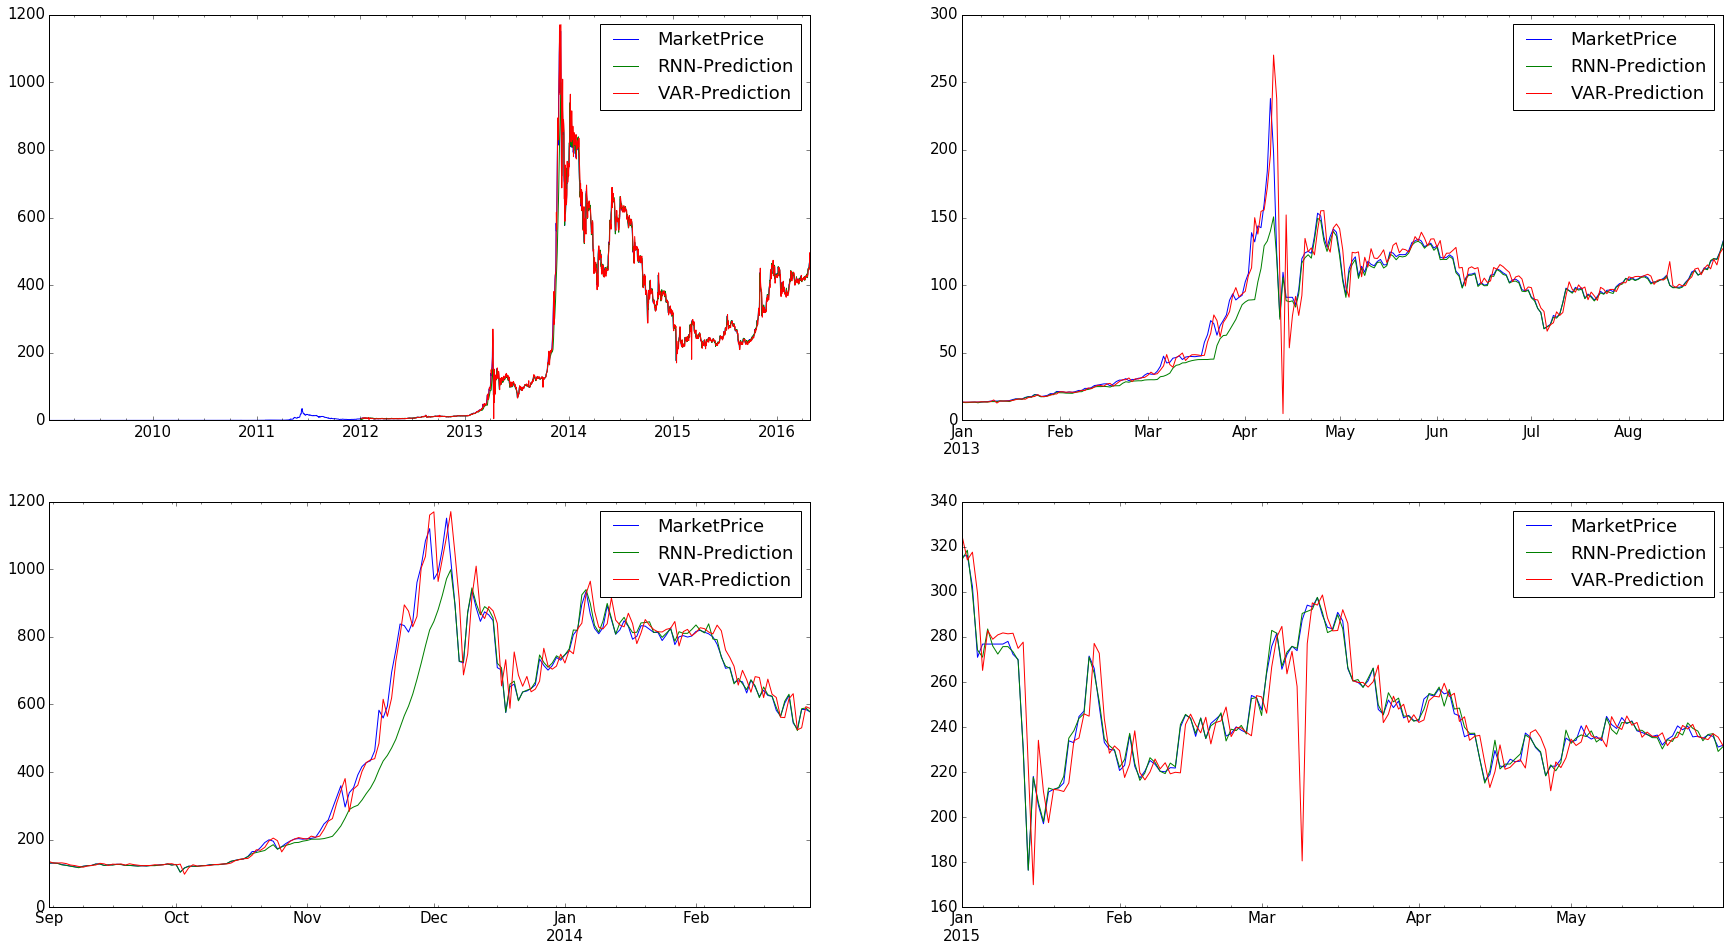
\includegraphics[width=1\linewidth]
    {gfx/predictions}}
  \caption{Predictions models and \textit{MarketPrice} true values in
    the same chart.}
  \label{fig:predictions}
\end{figure}

The main accuracy measure used is \textit{mean absolute error (MAE)},
shown in \autoref{eq:mae-expression}, averages the absolute error
produced for every prediction done with a particular model. This error
measure has the characteristic of represent quantities in the same
unit as the original variable and that is easily understandable.

\begin{equation}
  \begin{aligned}
    \label{eq:mae-expression}
    \textit{Mean Absolute Error: MAE} & =
    \frac{1}{n} \sum_{i=1}^{i=n} |e_i|\\
    e_i & = y_i - \hat{y}_i
  \end{aligned}
\end{equation}

In \autoref{tab:forecast-accuracy-measures} we present another error
measures to compare the predictions made by \textit{VAR} and
\textit{RNN}. The next accuracy measure to \textit{MAE} is
\textit{mean squared error (MSE)}, shown in
\autoref{eq:mse-expression}, which doesn't present the prediction
errors in the same unit, but has the feature of giving more importance
to bigger errors, than smaller ones. To see how this two measures
gives us different information about the same data we can see in
\autoref{tab:forecast-accuracy-measures} that, while \textit{RNN}'s
\textit{MAE} is lower than \textit{VAR}'s \textit{MAE}, the
\textit{RNN}'s \textit{MSE} is bigger than \textit{VAR}'s. That is
because \textit{RNN} errors are bigger and at the same time it has
less small errors. That can be clearly seen in
\autoref{fig:comparison-histogram-prediction-errors}.

\begin{equation}
  \begin{aligned}
    \label{eq:mse-expression}
    \textit{Mean Squared Error: MSE} & = \frac{1}{n} \sum_{i=1}^{i=n} e_i^2\\
    e_i & = y_i - \hat{y}_i
  \end{aligned}
\end{equation}

\begin{table}[bth]
  \myfloatalign
  \small
  \begin{tabularx}{\textwidth}{Xcc}
    \toprule \tableheadline{Measure Type} &
    \tableheadline{RNN Value}
    & \tableheadline{VAR Value} \\
    \midrule
    \textit{Mean absolute error (MAE)} & $5.4$ & $8.57$ \\
    \textit{Mean squared error (MSE)} & $638.55$ & $367.82$ \\
    \textit{Mean absolute percentage error (MAPE)} & $3.19$ & $3.46$ \\
    \textit{Theil's U statistic} & $0.47$ & $0.03$ \\
    \bottomrule
  \end{tabularx}
  \caption{Forecast accuracy measures}
  \label{tab:forecast-accuracy-measures}
\end{table}

Another accuracy measure used is \textit{mean absolute percentage
  error (MAPE)}, defined in \autoref{eq:mape-expression}. This measure
is useful when there are several scales, for example if the models are
run over different data-sets. This measure have the disadvantage of
being undefined for $y_i = 0$, and that it puts a heavier penalty on
negative errors than on positive errors.

\begin{equation}
  \begin{aligned}
    \label{eq:mape-expression}
    \textit{Mean Absolute Percentage Error: MAPE} & = \frac{1}{n}
    \sum_{i=1}^{i=n} \frac{100 \times e_i}{y_i} \\
    e_i & = y_i - \hat{y}_i
  \end{aligned}
\end{equation}

Finally we \textit{Theil's U statistic} which is defined in
\autoref{eq:theils-u-statistic}. This measure compares a forecast
model to the actual model. Is the ratio of the 1-step-ahead
\textit{MSE} for a given forecast relative to that of a random walk
forecast. If \textit{Theil's U statistic} is less than 1 then the
forecasting technique is better than guessing, if is exactly 1 then is
about as good as guessing and if it is more than 1 the forecasting
technique is worse than guessing.

\begin{equation}
  \begin{aligned}
    \label{eq:theils-u-statistic}
    \textit{Theil's U statistic} & = \sqrt{\frac {\displaystyle\sum_{t
          = 1}^{n - 1} \left( \frac{\hat{y}_{t+1} - y_{t+1}}{y_t}
        \right)^2} {\displaystyle\sum_{t = 1}^{n - 1} \left(
          \frac{y_{t+1} - y_t}{y_t} \right)^2}}
  \end{aligned}
\end{equation}

We can see in \autoref{tab:forecast-accuracy-measures} that the value
of \textit{Theil's U statistic} for \textit{RNN} is greater than that
of \textit{VAR} which can be understood as \textit{RNN} being closer
to $1$, so it's a worse forecasting technique than \textit{VAR} that
is closer to $0$.


[[[Analysis]]]

\begin{figure}[bth] \myfloatalign {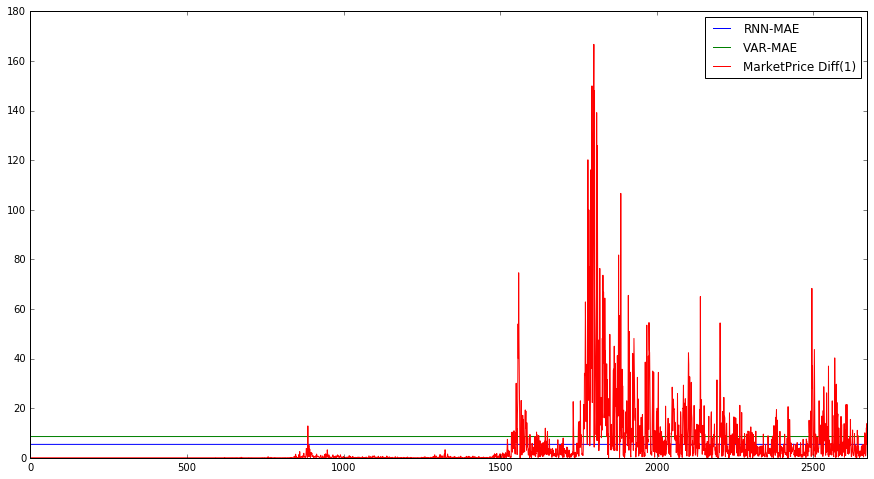
\includegraphics[width=1\linewidth]
{gfx/comparison-mae-with-diffs}}
  \caption{Comparison of \textit{VAR}-MAE value with
\textit{MarketPrice} first difference values.}
  \label{fig:comparison-mae-with-diffs}
\end{figure}

\begin{figure}[bth] \myfloatalign {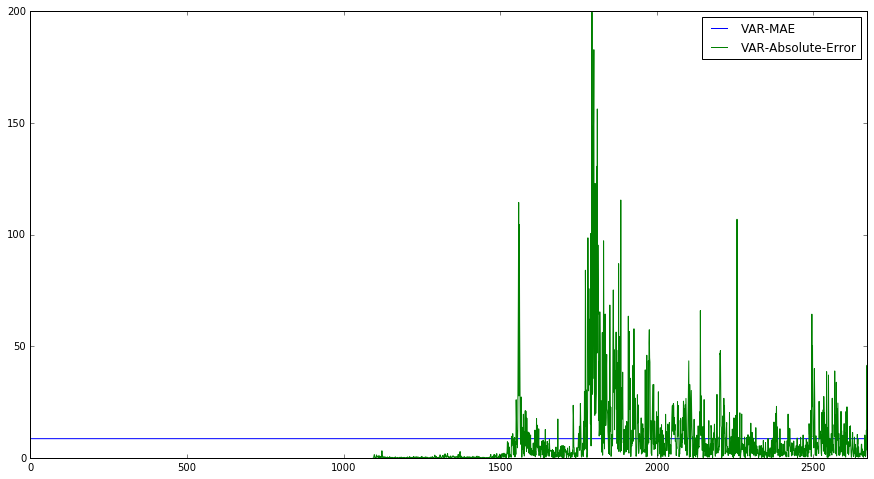
\includegraphics[width=1\linewidth]
{gfx/comparison-var-mae-with-var-absolute-error}}
  \caption{Comparison \textit{VAR}-MAE with absolute \textit{VAR}
errors.}
  \label{fig:comparison-var-mae-with-var-absolute-error}
\end{figure}

\begin{figure}[bth] \myfloatalign {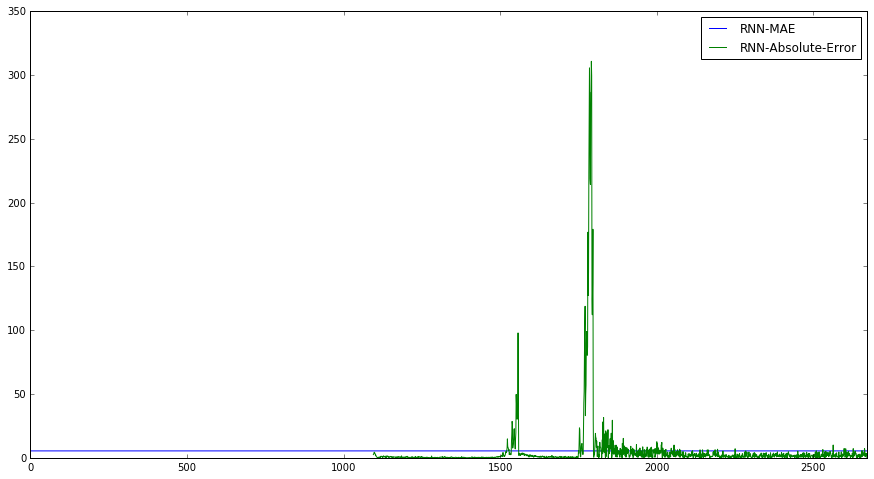
\includegraphics[width=1\linewidth]
{gfx/comparison-rnn-mae-with-rnn-absolute-error}}
  \caption{Comparison \textit{RNN}-MAE with absolute \textit{RNN}
errors.}
  \label{fig:comparison-var-mae-with-var-absolute-error}
\end{figure}

\begin{figure}[bth] \myfloatalign {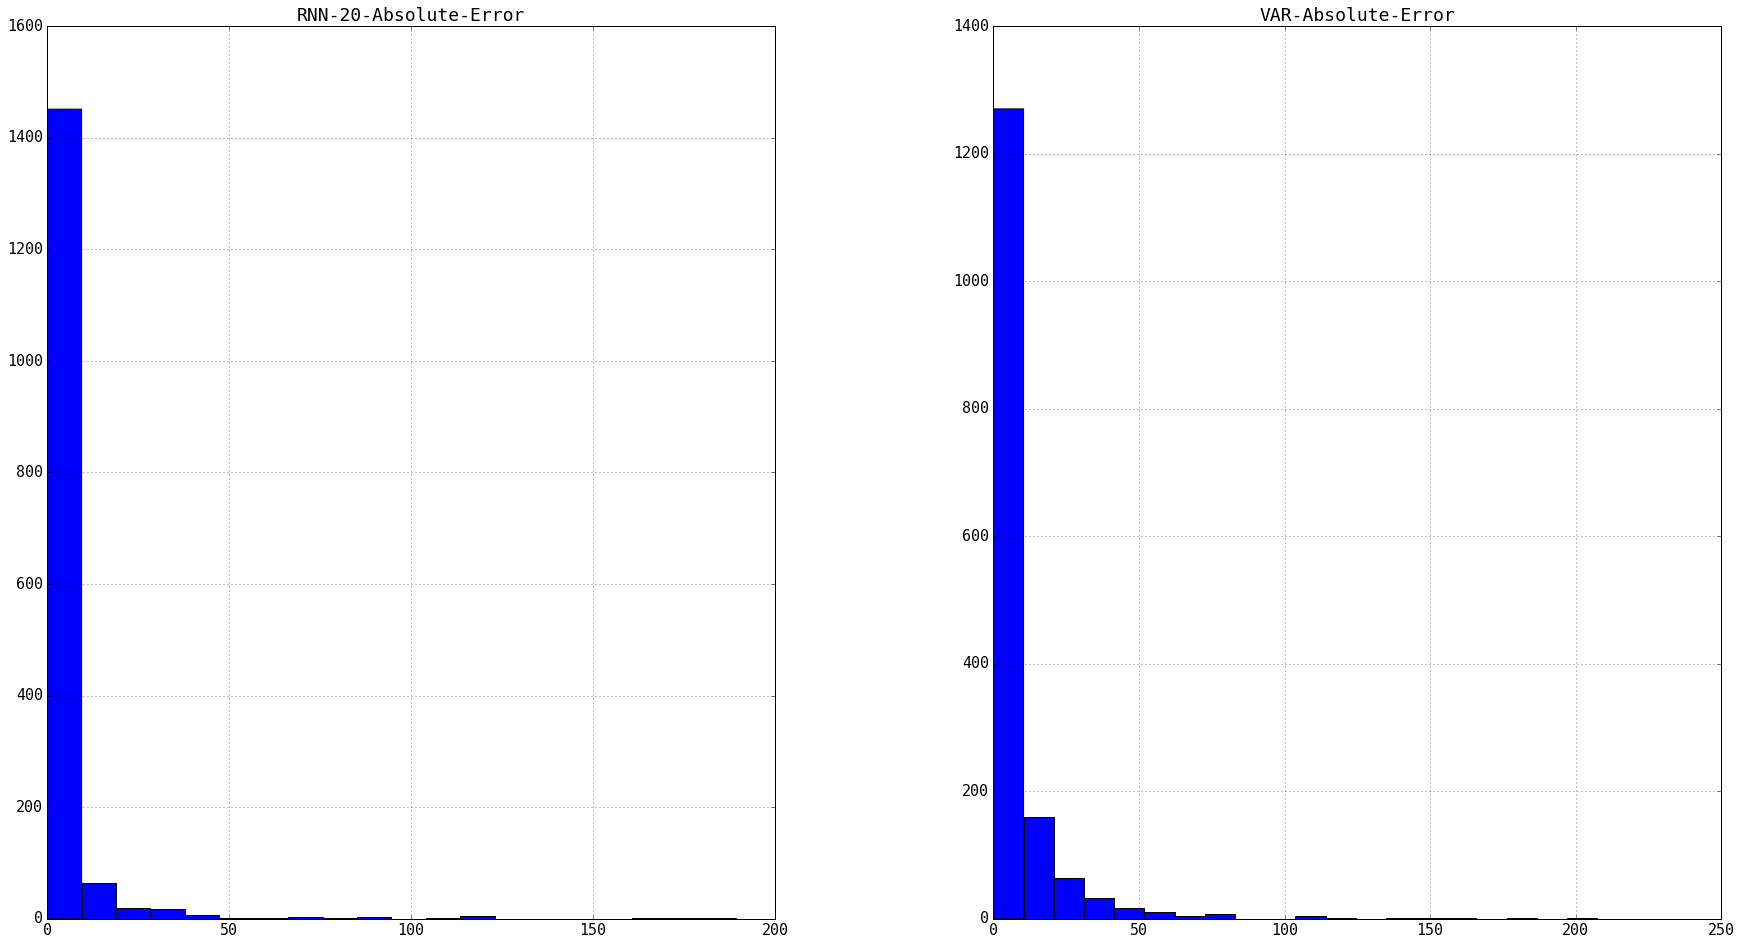
\includegraphics[width=1\linewidth]
{gfx/comparison-histogram-prediction-errors}}
  \caption{Histogram of \textit{RNN} absolute errors and \textit{VAR}
absolute errors.}
  \label{fig:comparison-histogram-prediction-errors}
\end{figure}

%---------------------------------------------------------------------
%---------------------------------------------------------------------
%---------------------------------------------------------------------

%\enlargethispage{2cm}

%------------------------------------------------

%%% Local Variables: %%% mode: latex %%% TeX-master: "../main" %%%
End:
